\section{Quantum Key Distribution}
Il QKD (Quantum Key Distribution) è una tecnologia che sfrutta l'entanglement quantistico, insieme alla trasmissione di bit su di un canale non sicuro, per scambiare una chiave comune a trasmettitore e ricevitore per una comunicazione cifrata e \textbf{simmetrica}.

\begin{info}
\textbf{Cenni di Cifratura}\\
Il significato di cifratura \textbf{simmetrica} è che, con la stessa chiave, riesco sia a cifrare che a decifrare un messaggio. A differenza, invece, della cifratura \textbf{asimmetrica}, dove la chiave per decifrare e per cifrare sono diverse. Per comprendere, ad alto livello, il funzionamento di tali meccanismi di cifratura, visualizzare l'immagine [\ref{img:cifratura}].
\end{info}

\begin{figure}[H]
\centering
\subfloat[][]{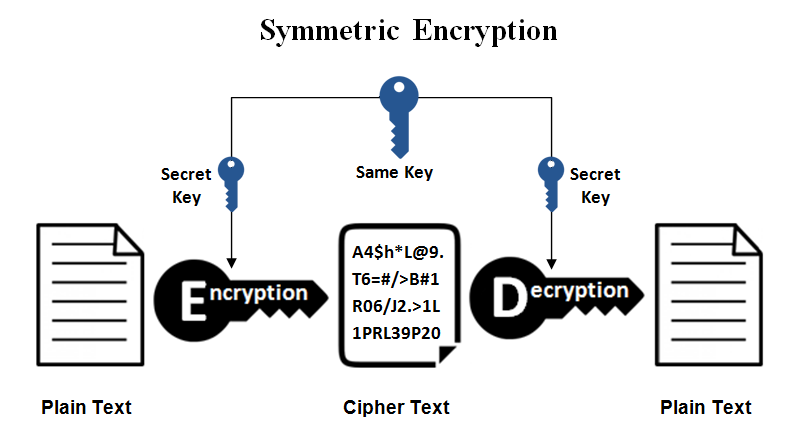
\includegraphics[width=.5\textwidth]{fig/Chapter-2/chapter-2/symmetric-encryption.png}}
\subfloat[][]{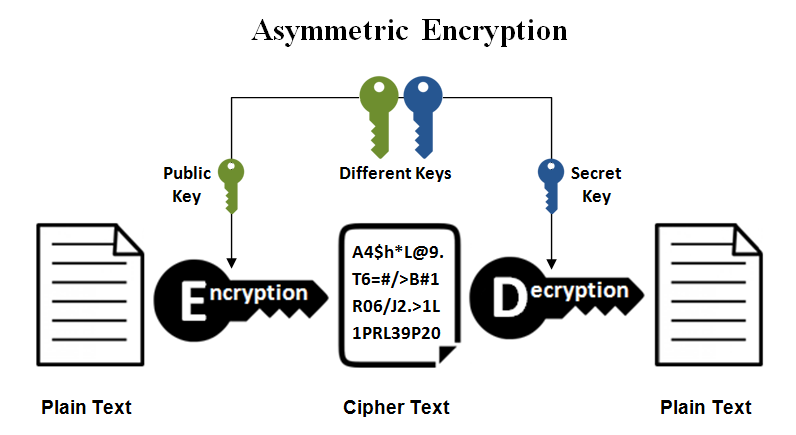
\includegraphics[width=.5\textwidth]{fig/Chapter-2/chapter-2/asymmetric-encryption.png}}

\caption{Cifratura simmetrica ed asimmetrica}\label{img:cifratura}
\end{figure}

Il \textbf{Quantum Computing} ha reso più vulnerabili gli odierni algoritmi di cifratura. Questo perché tali algoritmi basano la loro complessità sulla complessità computazionale molto elevata che viene richiesta per brute-forzare una chiave. In particolare:
\begin{itemize}
    \item \textbf{L'algoritmo di Shor}: Tale algoritmo permette di poter fattorizzare un numero intero in numeri primi è una minaccia importante per gli algoritmi a chiave asimmetrica. Tale algoritmo richiede molti qubit per essere eseguito, ma nonostante tutto è comunque potenzialmente pericoloso. Questo succede perché nella cifratura a chiave asimmetrica le chiavi che vengono utilizzare sono comunque collegate matematicamente
    
    \item \textbf{L'algoritmo di Grover}: Tale algoritmo permette di poter cercare un elemento all'interno di una lista con il brute force. Questo algoritmo può essere pericoloso per gli algoritmi a chiave simmetrica. 
\end{itemize}

Entrambe le soluzioni precedenti portano ad uno speed-up degli algoritmi per "bucare" tali sistemi. 

\begin{warn}
La comunità internazionale, accortasi del problema, in particolare per le comunicazioni asimmetriche, ha deciso di utilizzare degli algoritmo "\textbf{quantum-proof}" che sono stati chiamati algoritmi della \textbf{Post-Quantum Cryptography}, che invece cerca di sfruttare dei problemi matematicamente impossibili. O se non impossibili, non risolvibili ne da un computer classico ne da un computer quantistico
\end{warn}

\subsubsection{I fondamenti del QKD}
Il QKD cerca di sfruttare due fondamenti principali per la quantum information, ovvero:
\begin{itemize}
    \item Il teorema del \textbf{No-Cloning}
    \item Il \textbf{Postulato della Misura Quantistica}
\end{itemize}

Immaginiamo che Alice e Bob debbano comunicare tra di loro, vogliono sfruttare il QKD per distribuire la chiave simmetrica che poi andranno ad utilizzare per la loro comunicazione in modo classico. Pertanto quello che si va ad effettuare è sfruttare la misurazione su diverse coppie EPR, per poi scambiarsi le modalità di misura, da cui si decreterà poi la chiave (il metodo sarà esplorato meglio nelle prossime slide). La cosa importante è capire che per un eventuale attaccante che vorrà provare ad effettuare il man in the middle, sarà impossibile intromettersi all'interno di una comunicazione (non come nel mondo classico, dove con un cavo ethernet o con scheda wifi in modalità monitor, mediante wireshark, posso visualizzare i pacchetti letti dall'interfaccia, e provare ad effettuare attacchi di diverso tipo).

Se qualcuno provasse ad introdursi all'interno della comunicazione, non potrebbe farlo senza portare all'interno del sistema un disturbo. Questo è dimostrabile anche matematicamente come di seguito

\begin{info}
Per dimostrare che un man in the middle non possa entrare all'interno della comunicazione senza introdurre un disturbo, immaginiamo per assurdo che possa farlo. Pertanto ipotizzando che \(\ket{\psi}\) e \(\ket{\varphi}\) siano due stati non ortogonali su cui Eve(l'intruso) sta provando ad ottenere informazione. Di conseguenza, per non inserire disturbo, EVE effettuerà un'operazione unitaria tra \(\ket{\psi}\) o \(\ket{\varphi}\) con un'ancilla preparata in uno stato standard \(\ket{u}\). Assumendo che tale processo non disturbi gli stati, nei due casi si ottiene:
\[
\ket{\psi}\ket{u}\rightarrow \ket{\psi}\ket{v}
\]
\[
\ket{\varphi}\ket{u} \rightarrow \ket{\varphi}\ket{v'}
\]

Eve vuole che \(\ket{v}\) e \(\ket{v'}\) siano diversi per poter ricavare qualche informazione. Dato che il prodotto interno è preservato attraverso le trasformazioni unitarie, si va ad impostare la seguente uguaglianza:
\[
\braket{v | v'} \braket{\psi | \varphi} = \braket{u | u} \braket{\psi | \varphi}
\]

Essendo \(\ket{\psi}\) e \(\ket{\varphi}\) due vettori non ortogonali per ipotesi, allora \(\braket{\psi | \varphi} \ne 0\), il che mi permette di poterli ignorare da ambo le parti dell'equazione, ottenendo:
\[
\braket{v | v'} = \braket{u | u} = 1
\]
\end{info}

Questo implica che \(\ket{v}\) e \(\ket{v'}\) debbano essere lo stesso vettore, il che si traduce che Eve per ottenere informazione deve per forza introdurre disturbi all'interno della comunicazione.


\subsection{Bennett Brassard 1984 (BB84)}
Tale protocollo è il primo protocollo, che sfruttando il no-cloning, cerca di rendere possibile la condivisione di una chiave di cifratura classica mediante tecnologie quantistiche. I passi che si vanno a seguire sono i seguenti:

\begin{enumerate}
\item Alice genera una prima stringa di bit randomici di una lunghezza arbitraria (seguendo il riferimento \cite{nielsen2010}, \((4+\delta)n\), tale stringa di bit è denominata dal testo come \(a\))
\item Alice sceglie un'altra stringa di bit, che andranno a definire la base di riferimento (\(0:\{\ket{0}, \ket{1}\}\) oppure per \(1:\{\ket{+},\ket{-}\}\), tale stringa, nel testo, viene denominata \(a\))
\item Alice va a preparare, rispetto alle due precedenti stringhe, i qubit per la comunicazione. Precisamente il sistema potrà essere visto come:
\[
\ket{\psi} = \bigotimes_{k=1}^{(4+\delta)n} \ket{\psi_{a_k b_k}}
\]

Dove i singoli qubit \(\ket{\psi_{a_k b_k}}\) vegono preparati in base ai valori della stringa \(a\) e della stringa \(b\) seguendo la regola per cui:
\begin{itemize}
    \item \(a_k=0, b_k=0\): \(\ket{\psi_{00}}=\ket{0}\)
    \item \(a_k=1, b_k=0\): \(\ket{\psi_{10}}=\ket{1}\)
    \item \(a_k=0, b_k=1\): \(\ket{\psi_{01}}=\ket{+}\)
    \item \(a_k=1, b_k=1\): \(\ket{\psi_{11}}=\ket{-}\)
\end{itemize}
Una volta preparati, li invia direttamente a Bob

\item Bob riceve i qubit inviati da Alice e lo annuncia (tipo un piccolo ack di ricezione). Una volta fatto questo, Bob procede a misurare i qubit seguendo le indicazioni di una stringa randomica che genera esso stesso (tale stringa, nel testo viene chiamata \(b'\))
\item Alice annuncia la stringa \(b\)
\item Bob annuncia la stringa \(b'\) (questa non viene citata nel testo, ma è necessaria per il funzionamento del protocollo)

\item Alice e Bob scartano ogni bit che Bob ha misurato con una base differente da quella con cui alice aveva preparato i qubit. Con una probabilità abbastanza alta, ci sono almeno \(2n\) bit mancanti (se non dovesse essere così, allora si interrompe il protocollo). Loro manterranno \(2n\) bit
\item Alice seleziona un sottoinsieme di \(n\) bit che andrà ad utilizzare per verificare se ci sia una interferenza portata da Eve, per poi dire a bob quali bit ha selezionato
\item Alice e Bob annunciano e comparano i valori degli n bit di check. Se più di un certo numero accettabile, sono diversi, allora si termina il protocollo
\item Alice e bob faranno una riconciliazione e un amplificazione di privacy sui restanti \(n\) bit per ottenere \(m\) chiavi condivise.
\end{enumerate}

Quello che accade dal passo 7 in poi è una verifica per comprendere se Eve ha introdotto più disturbo (rispetto anche a quello introdotto dall'eventuale canale tra Alice e Bob). Questo avviene selezionando un sottoinsieme dei bit che sono stati "concordati" tra i due, verificato che tali bit differiranno per una valore determinato di t bit. Tale verifica permetterà di capire se Eve si è introdotta con ulteriore disturbo o meno. 

Il difetto del BB84 è che, sfruttando l'invio dei qubit, richiede un'infrastruttura apposita. Precisamente, richiede dei trusted node su cui ci si ferma ad effettuare il protocollo per poi generare una serie di comunicazioni tra i trusted node fino a destinazione. Il motivo è dovuto al fatto che un fotone, nel mondo quantistico, per via del no-cloning, non può essere rigenerato, come nel modo classico, da un normale ripetitore.

\subsection{Ekert 1991 (E91)}
L'Ekert 1991 (o Ekert-91 o E91) è un'estensione del protocollo QKD con l'utilizzo di coppie EPR. Quello che principalmente cambia è la trasmissione dei qubit stessi.

Le regole dell'Ekert-91 sono semplici:
\begin{enumerate}
    \item Alice e Bob pre-distribuiscono delle coppie EPR tra di loro
    \item Alice e Bob scelgono randomicamente le basi lungo cui misurare i loro qubit delle coppie EPR (generazione di due stringhe randomiche per la scelta delle basi, sono esattamente \(b\) e \(b'\) incontrate nel BB84)
    \item Alice e Bob si condividono le stringhe che spiegano lungo che base hanno effettuato la misura (si condividono \(b\) e \(b'\))
    \item Dopo la condivisione, Alice e Bob mantengono solo i bit che corrispondono alla stessa misura, questo ne permette la perfetta generazione della chiave
\end{enumerate}


\subsection{Considerazioni sul QKD}
Il QKD, come visto precedentemente, richiede:
\begin{itemize}
    \item Nel caso del BB84, di dover trasmettere dei fotoni lungo delle linee. Essendo che i fotoni, all'interno delle fibre, vengono persi (su 10 fotoni, solo uno arriva a destinazione dopo 50 km, gli altri vengono perduti)
    \item Nel caso dell'E91 è la distribuzione di molte coppie EPR tra trasmettitore e ricevitore. Essendoci anche la tecnica di quantum swapping, questo non è complicato, ma richiederebbe la realizzazione di porte in tecnologia fotonica (non proprio facili da realizzare)
\end{itemize}

Nelle implementazioni reali, però, bisogna tenere conto di:
\begin{itemize}
    \item Rumorosità del canale quantistico
    \item Eavesdropper (rumore introdotto da Eve)
\end{itemize}

Con la presenza di tali problematiche, la chiave che Alice e Bob vogliono condividere può contenere dei mismatch non dovuti al protocollo, ma dovuti ai diversi rumori. Essendo che Alice e Bob non possono rivelare le loro chiavi (per ovvi motivi), l'unico modo è utilizzare delle specifiche tecniche di post-processing. Tra queste troviamo:
\begin{itemize}
    \item \textbf{Key sifting}: rivelare alcune delle chiavi condivise
    \item \textbf{Key reconciliation}: correzione dell'errore sulla chiave setacciata
    \item \textbf{Privacy amplification}: riduzione della chiave setacciata
\end{itemize}

\subsubsection{Key Sifting}
La tecnica del Key Sifting permette di capire l'entità dell'informazione che è stata "perduta" o disturbata durante la trasmissione. Questo avviene con la condivisione di parte della chiave che viene condivisa per essere confrontata. Una volta confrontata si decide se arrestare il protocollo in base al BER(Bit Error Rate) threshold. In particolare:
\begin{itemize}
    \item Se: BER osservato < BER threshold -> si può procedere con la key reconciliation
    \item Se: BER osservato >= BER threshold -> bisogna interrompere il protocollo, potenziale eavesdropper
\end{itemize}

Non è possibile distinguere, solo dal BER, se vi è la presenza di eavesdropper o meno, questo perché il disturbo non viene distinto da quello introdotto dal canale di comunicazione stesso

\subsubsection{Key Reconciliation}
Quello che viene fatto in questa fase è cercare di ridurre il numero di mismatch della chiave tra Alice e Bob. Per effettuare questa cosa vi è una problematica, condividere la chiave su un canale non sicuro risulta impossibile. Pertanto quello che si va ad effettuare è la suddivisione in blocchi della chiave ed il calcolo della parità tra di loro. Trovati i mismatch, si vanno a scambiare solo tali mismatch, dove la parità è diversa. 

Quello che solitamente si va ad effettuare è un mescolamento dei bit con un'applicazione di \(k\) volte il check di parità (seguendo queste chiavi mescolate). Questo permette di poter evitare casi in cui la sola parità non basti. Aumentando considerevolmente il numero di \(k\), la probabilità che le chiavi siano identiche aumenta (perché si riduce la probabilità di "errori nascosti").

La probabilità di errori nascosti si esprime come:
\[
p = 1 - \left(\frac{1}{2}\right)^k
\]
Tale tecnica non è molto difficile da implementare, ma questo non basta, essa ha anche dei contro che sono:
\begin{itemize}
    \item Quantità gigante di informazioni che trapelano su di un canale non sicuro
    \item delay molto grande per la correzione dell'errore
\end{itemize}

La soluzione a tali problemi risiede nell'utilizzare metodologie di error-correction più forti, come ad esempio: Turbo codes, LDPC codes, Polar codes.

\subsubsection{Privacy Amplification}
La key reconciliation è un'operazione che avvenendo su un canale non sicure, rende i "messaggi" si comunicazione tra Alice e Bob visibili, il che aggiungerà informazioni utili ad Eve per "decifrare" la chiave. Quindi Alice e Bob hanno bisogno di eliminare quanta più informazione sporcata, sia da Eve, che da eventuale rumore.

Bisogna quindi trovare il modo di effettuare delle operazioni di \textbf{Privacy Amplification}.
Assumendo che Alice e Bob condividano n-bit della chiave condivisa ed Eve ha t-bit della chiave ricavati (Alice e Bob non hanno idea di quali t bit siano). La domanda che quindi ci si pone è: è possibile che Alice e Bob possano usare la chiave corrente? Hanno bisogno di ricominciare il processo da capo?

Non è necessario ricominciare il processo. Alice e Bob possono generare una chiave segreta di (n-t) bit a partire dalla chiave condivisa di n bit. Pur non sapendo quali bit siano noti a Eve, possono stimare approssimativamente quanti sono (t). Applicano allora una funzione hash universale, scelta a caso e comunicata pubblicamente, che comprime la chiave mescolandone tutti i bit: la chiave risultante, più corta, è segreta per Eve e può essere usata per la cifratura